\documentclass[conference]{IEEEtran}
\IEEEoverridecommandlockouts
% The preceding line is only needed to identify funding in the first footnote. If that is unneeded, please comment it out.
\usepackage{cite}
\usepackage{amsmath,amssymb,amsfonts}
\usepackage{algorithmic}
\usepackage{graphicx}
\usepackage{textcomp}
\usepackage{xcolor}
\def\BibTeX{{\rm B\kern-.05em{\sc i\kern-.025em b}\kern-.08em
    T\kern-.1667em\lower.7ex\hbox{E}\kern-.125emX}}
\setlength{\parindent}{0pt}
\begin{document}

\title{Network Security Lab 4: Identifying IPv6 Addresses}

\author{\IEEEauthorblockN{Alexander Hoffmann}
\IEEEauthorblockA{\textit{ECE Paris}\\
Paris, France \\
alexander.hoffmann@edu.ece.fr}
}

\maketitle

\section{Identify the Different Types of IPv6 Addresses}
\subsection{Match the IPv6 address to its type}

\begin{center}
\begin{tabular}{ |c|c| } 
 \hline
 2001:0DB8:1:ACAD::FE55:6789:B210 & Global unicast address \\ 
 \hline
 ::1 & Loopback address \\ 
 \hline
 FC00:22:A:2::CD4:23E4:76FA & Unique-local address \\ 
 \hline
 2033:DB8:1:1:22:A33D:259A:21FE & Global unicast address \\ 
 \hline
 FE80::3201:CC01:65B1 & Link-local address \\ 
 \hline
 FF00:: & Multicast address \\ 
 \hline
 FF00::DB7:4322:A231:67C & Multicast address \\ 
 \hline
 FF02::2 & Multicast address \\ 
 \hline
\end{tabular}
\end{center}

\section{Examine a Host IPv6 Network Interface and Address}
\subsection{Check your PC IPv6 network address settings}

\begin{center}
\begin{figure}[h]
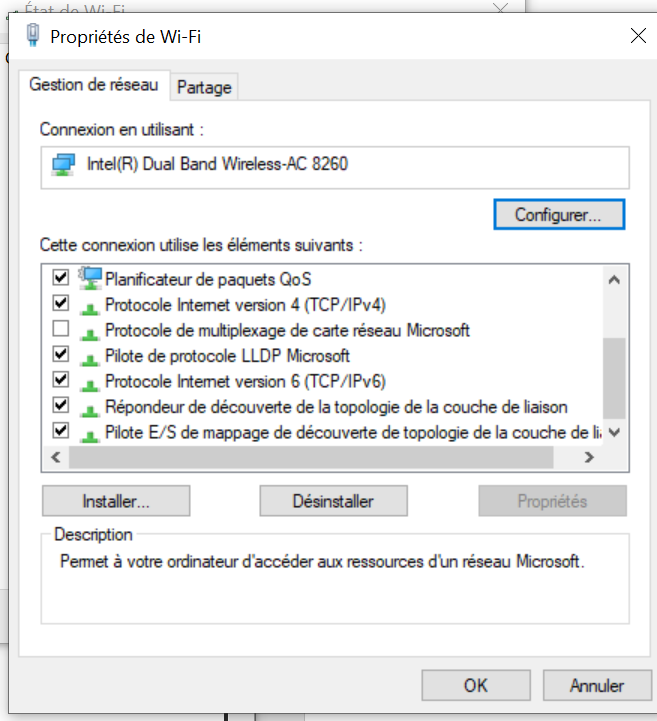
\includegraphics[scale=0.35]{resources/q1e.png}\
\caption{Configuration of the accounting server}
\label{server_acc}
\end{figure}
\end{center}

\begin{center}
\begin{figure}[h]
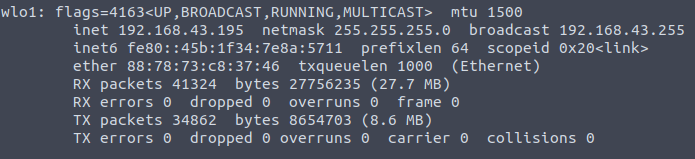
\includegraphics[scale=0.45]{resources/q1f.png}\
\caption{Configuration of the accounting server}
\label{server_acc}
\end{figure}
\end{center}

\textbf{i.} It indicates that there is no IPv6 enabled gateway router providing global address, local address, or subnet information on the network.

\textbf{f.} Answers will vary, but most likely they will be link-local addresses also.

\section{Practice IPv6 Address Abbreviation}
\subsection{Study and review the rules for IPv6 address abbreviation}
1)2002:0EC0:0200:0001:0000:04EB:44CE:08A2
2002:EC0:200:1::4EB:44CE:8A2\\

2)FE80:0000:0000:0001:0000:60BB:008E:7402
FE80::1:0:60BB:8E:7402\\

3)FE80::7042:B3D7:3DEC:84B8
FE80:0000:0000:0000:7042:B3D7:3DEC:84B8\\

4)FF00::
FF00:0000:0000:0000:0000:0000:0000:0000\\

5)2001:0030:0001:ACAD:0000:330E:10C2:32BF
2001:30:1:ACAD::330E:10C2:32BF\\

\end{document}
